\chapter{Multiplication implementation}\label{Chpater_Impl_mul}
\section{Introduction}
The purpose of this chapter is to introduce and explain the hardware implementation of Booth's signed multiplication algorithm.
This algorithm is presented in the form of pseudo-code in \autoref{code:booth_mul}, where $N$ is the length of multiplicand $A$ and multiplier $B$, so their product $P$ will be $2 \cdot N$ bits long; in our processor $N = 32$.
The contents of the look-up table (\textit{LUT}) are shown in \autoref{tab:booth_mul_lut}.

The multiplication circuit is split into two sub-units: a controller which keeps track of how many intermediate products still need be computed, and a datapath which actually performs the necessary operations.

\begin{lstlisting}[label={code:booth_mul}, caption={The C-like psuedo code implementing the radix-4 booth multiplication}, language=C]
int booth_mul(int A, int B) {
    i = 0;
    P = 0;
    
    B = B << 1;

    while (i < N/2){
        factor = LUT(B[2:1])
    
        P = P + A * factor;
        A = A << 2;
        B = B >> 2;
        i = i + 1;
    }

    return P;
}
\end{lstlisting}
\begin{table}[]
    \centering
    \begin{tabular}{|c|c|c|c|}
        \hline
         B[2] & B[1] & B[0] & factor\\
         \hline
          0 & 0 & 0 & 0\\
         0 & 0 & 1 & 1\\
         0 & 1 & 0 & 1\\
         0 & 1 & 1 & 2\\
         1 & 0 & 0 & -2\\
         1 & 0 & 1 & -1\\
         1 & 1 & 0 & -1\\
         1 & 1 & 1 & 0\\
         \hline 
    \end{tabular}
    \caption{Contents of the LUT used in Booth's algorithm}
    \label{tab:booth_mul_lut}
\end{table}

\section{Controller}
A simplified view of the states of the controller is shown in \autoref{fig:booth_mul_controller} (some control signals are not shown for brevity).
It's a very simple controller because the operations executed at each clock cycle are always the same.

\begin{figure}
    \centering
    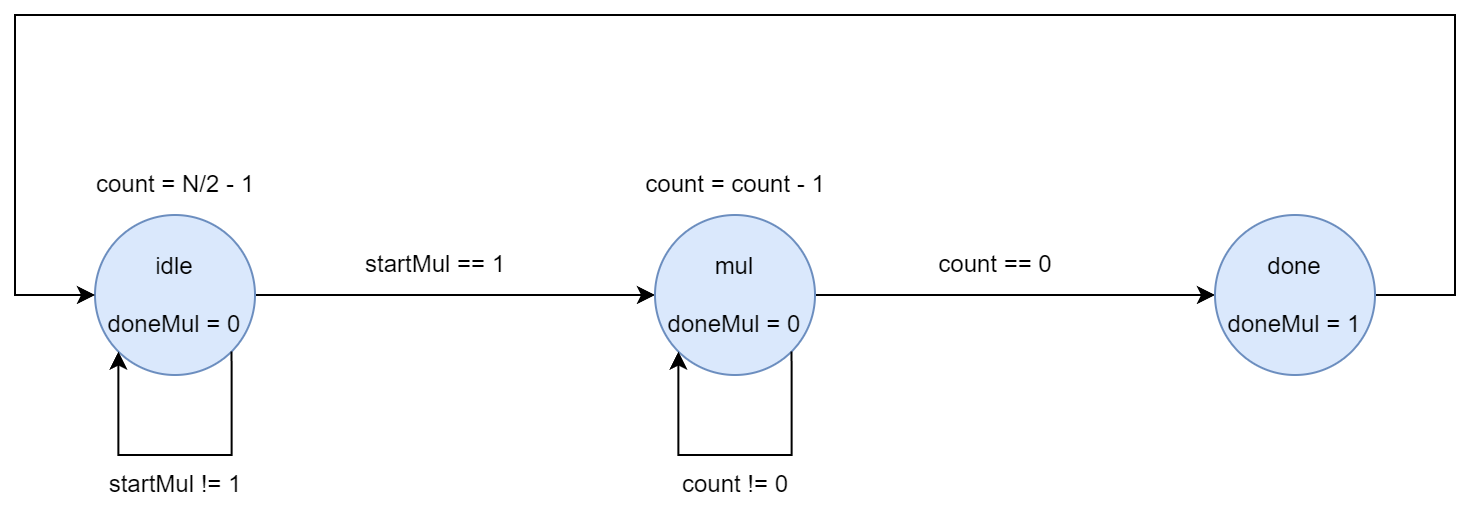
\includegraphics[width=0.9\linewidth]{images/boothControllerSimplified.png}
    \caption{Simplified sate diagram of the controller}
    \label{fig:booth_mul_controller}
\end{figure}

Upon reset, the controller is initialised to the \texttt{idle} state and waits for the processor's control unit to assert the \texttt{startMul} signal, thus requesting a multiplication to be performed.

After that, the controller moves into the \texttt{mul} state and asserts the control signals needed to compute the intermediate products.
Since the multiplicand and multiplier are $N = 32$ bits long, the controller stays in this state for $N / 2 - 1 = 15$ clock cycles.

After the final product has been computed the controller moves to the \texttt{done} state: the purpose of this state is to let the controller know that the product is ready, and to do so the \texttt{doneMul} signal is raised (no other operation is performed).

The result is available for one clock cycle: after that the controller goes back to the \texttt{idle} state and will wait to be instructed to run the multiplication again.

\section{Datapath}
The datapath, just like the controller, is very simple and is shown in \autoref{fig:booth_mul_datapath}.
Its purpose is to compute the intermediate products, so it implements the body of the \textit{while} loop as it was shown in the code.

\begin{figure}
    \centering
    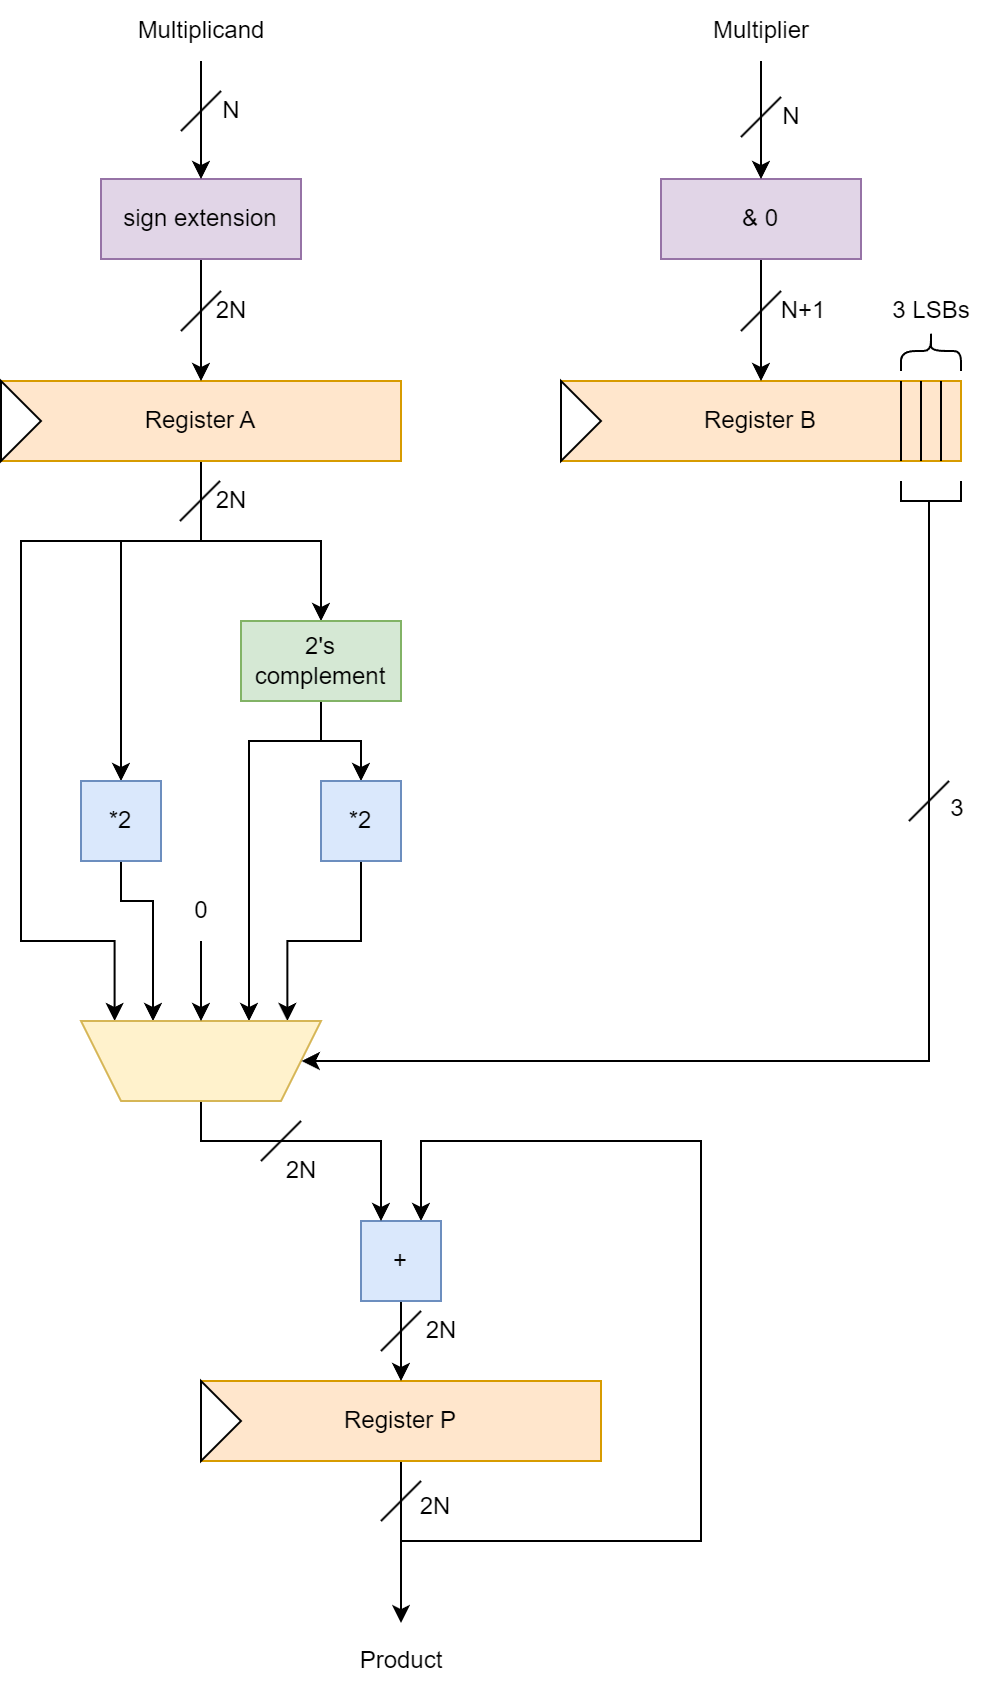
\includegraphics[width=0.8\linewidth]{images/boothDatapath.png}
    \caption{Diagram of the datapath}
    \label{fig:booth_mul_datapath}
\end{figure}

While the controller is in the \texttt{idle} state, the multiplicand $A$ is sign-extended to $2 \cdot N = 64$ bits to match the length of the product $P$ while a zero is appended to the multiplicand $B$'s LSB, which is equivalent to left-shifting $B$ ny one position.

The main difference between this implementation and the code is in the absence of the LUT: it is replaced by computing in parallel $0$, $\pm A$, $\pm 2 \cdot A$ and using $B$'s LSBs as the selection signal of a multiplexer, without involving a memory component.
The output of the multiplexer, which is $A \cdot \text{factor}$, is summed to $P$'s current value to generate the next partial product, which will be written to the product's register at the next rising edge of the clock.

It's important to know that both $A$'s and $B$'s registers are shift registers: $A$'s register left-shifts the multiplicand by two positions at each clock cycle, while $B$'s register right-shifts the multiplier by the same amount.

The value in the register $P$ is accessed as-is from the outside.